\subsection{Aeroponics}
\label{sec:aeroponics}

\textbf{Purpose}: Delivers plant nutrients and pH- and temperature-controlled water to the roots via a fine mist.

\textbf{Function}:
\begin{itemize}
    \item \textbf{Inputs}: Reverse osmosis water\footnote{RO water has no dissolved nutrients and a neutral pH of 7.0. This enables easier and more reliable calculations. In addition, it has no particulate or minerals, minimizing the chances of nozzle clog.} under positive pressure, concentrated pH up \& down solutions and nutrient solutions, nozzle delivery on/off control (\ref{sec:automation}), pH and nutrient solution ratios as control signals (dosing pump speeds; \ref{sec:automation}), water thermoregulation control signal (\ref{sec:automation})
    \item \textbf{Outputs}: pH- and nutrient-controlled water mist (50 micron mean droplet diameter)
\end{itemize}

\textbf{Method}:
\begin{enumerate}
    \item \textit{Setup}:
    \begin{enumerate}
        \item Hook up water, solution, and signal inputs;
        \item Connect the quick-disconnect fitting;
        \item Calibrate pressure, temperature sensors to atmospheric;
        \item Enable water input to prime system (if known pressure/temperature, calibrate sensors);
        \item Mount container, connect runoff collection line to recycling port;
    \end{enumerate}
    \item \textit{Testing}:
    \begin{itemize}
        \item Temperature, pressure sensors communicate as expected.
        \item No leaks at any connections under a) source pressure, b) fully pressurized.
        \item Pump actuates and auto-shuts off as expected, and is able to deliver the required pressure.
        \item All components, tubing, and connectors/fittings withstand full pressurization.
        \item Solenoid is normally closed, withstands full pressurization, and opens when power is applied.
        \item Quick-disconnect operates as intended at full pressurization without leaks.
        \item Nozzles produce even-distribution full-cone mist.
        \item Manual and actuated valves operate as intended.
        \item Runoff container is sealed, and runoff collection operates as intended.
    \end{itemize}
    \item \textit{Process}:
    \begin{enumerate}
        \item Water is pressurized to constant 80psi;
        \item Heat is added to or removed from the water;
        \item Temperature and pressure of the water is read (feedback);
        \item Nutrient and pH solutions are mixed in-line at an adjustable ratio\footnote{I.e. add X mL of nutrient solution Y per mL water to achieve Z ppm, or add A mL of pH down solution per mL water to achieve a pH of B.};
        \item Flow to nozzle is controlled (on/off);
        \item Nozzle turns pressurized water into mist;
        \item Runoff is contained by a water-tight container, and collected for recycling;
    \end{enumerate}
    \clearpage
    \item \textit{Shutdown}:
    \begin{enumerate}
        \item Power down the pump and thermoregulation unit;
        \item Close the nutrient and pH solution valves;
        \item Close the source shutoff valve;
        \item Open the drain valve, and allow the system to depressurize completely;
        \item Re-open the source shutoff valve and flush the system with fresh water;
        \item Power down the solenoid;
        \item Collect all remaining runoff;
        \item Disconnect the quick-disconnect fitting;
        \item Disconnect the inputs;
    \end{enumerate}
\end{enumerate}

\textbf{Features}:
\begin{itemize}
    \item \textit{Water Source}: Input for ambient reverse-osmosis water.
    \item \textit{Manual Source Shutoff Valve}: Ball valve.
    \item \textit{Diaphragm Pump}: Self-priming, auto-shutoff at 80psi. Power is controlled by a relay.
    \item \textit{Inline Thermoelectric Water Heater/Cooler Block}: Aluminum water block heat pump. See Section \ref{sec:airthermoregulation}.
    \item \textit{PID Control Loop}: A propotional-integral-derivative (PID) control loop enables increased accuracy (see equation \ref{eqn:pid}, section \ref{sec:airthermoregulation}).
    \item \textit{Solution Injection Manifold}: A manifold of parallel in-line injectors, allowing for on-demand adjustment of mixing ratios for nutrient and pH solutions. Comprises:
    \begin{itemize}
        \item \textit{Manifold}: Splits the water line into a set of parallel branches with inline tees to enable solution injection.
        \item \textit{Dosing Pumps}: Stepper-motor driven custom peristaltic pumps deliver solutions at a controlled rate/ratio (one per solution). Toleranced to prevent backflow at pressure. % TODO more details (tubing type, washers, bearings, etc.) w/ part numbers
        \item \textit{Nutrient Solutions}: Aqueous. Highly concentrated. Selectable as part of the program (\ref{sec:automation})\footnote{Many different solutions can be combined (according to solubility laws, pH requirements, etc.).}, and may include any of:
        \begin{itemize}
            \item Bioavailable nonmetals (ammonia, ammonium, nitrates, nitrites, phosphates, sulfates, etc.)
            \item Bioavailable metals (potassium, etc.)
            \item Minerals (magnesium, calcium)
            \item Other trace elements
            \item Custom solutions (i.e. fungicides/algicides, descaling solutions)
        \end{itemize} 
        \item \textit{pH Adjustment Solutions}\footnote{\textit{NOTE:} Ionic composition of pH solutions should be considered in the understanding of the nutrient composition (i.e. phosphic acid results in phosphate ions in spray)}: Aqueous. Highly concentrated. One for pH up (>8), one for pH down (<6).
        \item \textit{Solution Storage Containers}: Opaque, insulated, chemical-safe, refillable cartridges. Prevent degradation of solution compounds over time via light or heat.
        \begin{itemize}
            \item \textit{Fill Level Sensors}: Depth sensors measure fill level of container. Notifies user to refill.
        \end{itemize}
    \end{itemize}
    \item \textit{Water Temperature Sensor}: Tee-fitted. Informs the \textbf{PID control loop}. See Section \ref{sec:airthermoregulation}.
    \item \textit{Accumulator Tank}: Uses an air bladder to maintain and stabilize pressure.
    \item \textit{Pressure Sensor}: Allows for shutoff of pump in case of emergency.
    \item \textit{Drain Valve}: Tee-fitted ball valve. Allows the system to be depressurized and drained.
    \item \textit{Solenoid Valve}: Controls delivery to the nozzles to enable on-demand misting.
    \item \textit{Grow Tray Quick-Disconnect}: Connectors between aeroponics supply and nozzles that allow for quick disconnection with auto-shutoff so the trays may be removed.
    \item \textit{Nozzle}: Mounted to grow tray, pointed at plant roots. 80psi water through a 0.4-0.6mm orifice produces 5-50 micron water droplets, optimal for plant growth.
    \item \textit{Root-Zone Container}: Watertight container that encapsulates the entire root zone. Made of a woven waterproof composite fabric (CT5K.18 mylar with Dyneema, 33.89g/m${}^2$), chosen for high strength-to-weight ratio (15x that of steel) and natural no-coating food-safe waterproof quality \cite{dyneema}. Mounted and \textbf{sealed} to the grow tray with a drawstring for easy root zone access. Provides water supply and runoff collection ports.
\end{itemize}

\textbf{Figures}

\begin{figure}[h!]
    \centering
    \frame{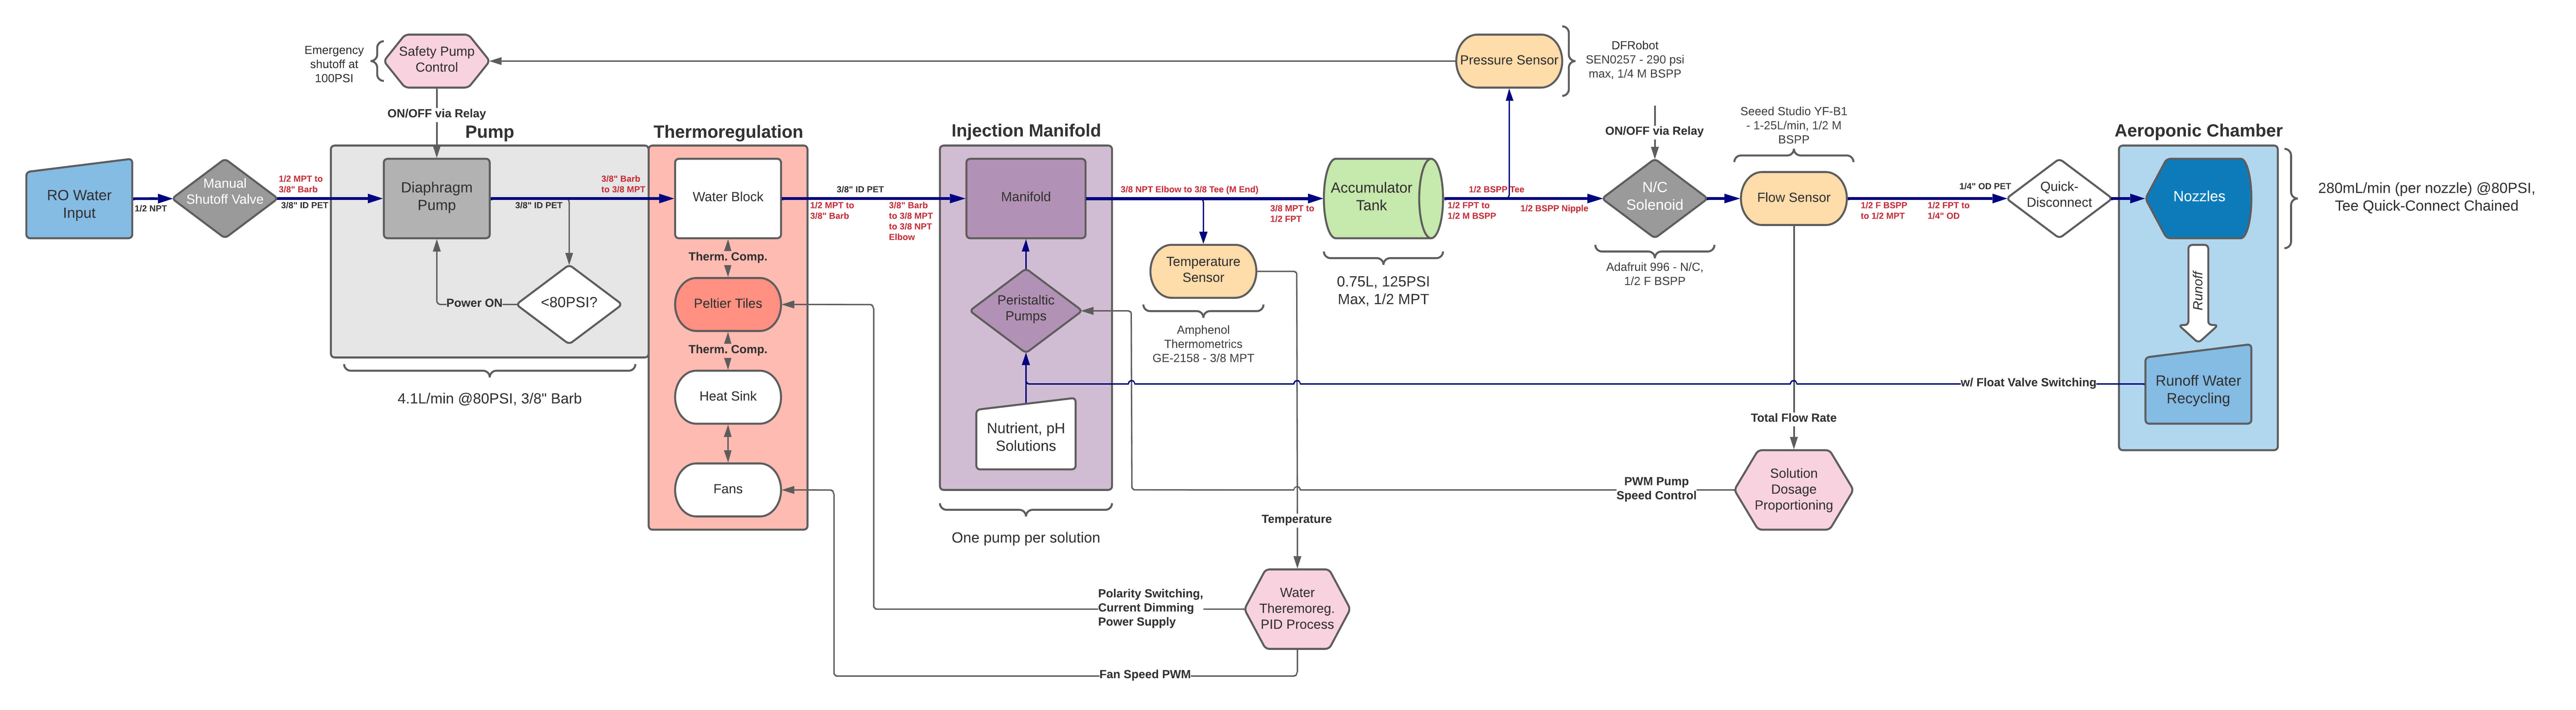
\includegraphics[width=\textwidth]{../assets/figures/aeroponics_plumbing.png}}
    \caption{Aeroponics plumbing diagram.}
    \label{fig:aeroponics_plumbing}
\end{figure}

\begin{figure}[h!]
    \centering
    \frame{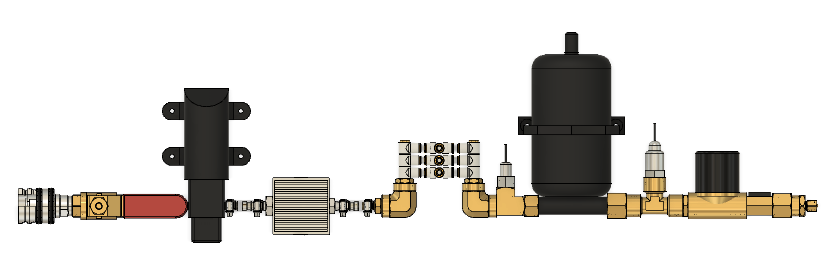
\includegraphics[width=\textwidth]{../assets/figures/aeroponics_supply.png}}
    \caption{Aeroponics supply system.}
    \label{fig:aeroponics_supply}
\end{figure}

% TODO Pump model figure

\clearpage